\documentclass[a4paper,11pt,twoside]{IT-CNEA}
\usepackage[utf8]{inputenc} % para cambiar el encoding
\usepackage{multicol}

%%%%%%%%%%%%%%%%%%%%%%%%%%%%%%%%%%%%%%%%%%%%%%%%%%%%%%%%%%%%%%%%%%%%%%%%%%%
%               Parametros principales del documento                      %
%%%%%%%%%%%%%%%%%%%%%%%%%%%%%%%%%%%%%%%%%%%%%%%%%%%%%%%%%%%%%%%%%%%%%%%%%%%

% Titulo
\titulo{Propagación de ruido en sistema LTI}
%
% Titulo alternativo para el encabezado
\alttitulo{Elementos de matemáticas aplicada para aplicaciones tecnlógicas}

% Autores
\autores{Augusto Conrado Sardá}{}

% Revisores
\revisores{Jose Relloso}{Agustín Casquero}{}

% Revision de calidad
\calidad{}

% Aprobacion
\aprobacion{}

%Objetivo
\objetivo{}
% Alcance
%\alcance{}

% Numero de informe tecnico
\numeroIT{TP Nº0}
% Metadatos para pdf
\hypersetup{
    pdfauthor={Augusto Conrado Sardá},
    pdftitle={Propagación de ruido en sistema LTI},
    pdfkeywords={},
    pdfcreator={},
    pdfsubject={}    
    }
    
% Autores de revisiones
%\definechangesauthor[name={Johann Sebastian Mastropiero}, color=blue]{mas}
\usepackage{units}
\usepackage{fancyvrb}
\begin{document}
    % Creacion de la caratula
%    \portada    
    % Creacion del indice
    \tableofcontents       
    % Comienzo del desarrollo del documento
    \printnomenclature[2cm]

\newpage  
\section{MEMORIA DESCRIPTIVA}
En el presente informe se analiza la respuesta de un sistema lineal e invariante en el tiempo a una entrada estocástica. La motivación surge de que en cualquier sistema que se desea controlar, se deberán medir las variables de interés. Para esto será necesario utilizar los sensores pertinentes, cuya medición estará sujeta a ruido, ya sea inherente a su principio de funcionamiento o a condiciones externas. Por lo tanto, asumiendo que la medición presentará ruido, se puede conocer como responderá el sistema frente a este. 
\par Se utiliza como ejemplo de un sistema de control de altitud de \cite{Sidi}. El modelo del sistema se muestra en la Fig. Nº\ref{fig:ModeloControlAltitudSidi}, donde se supone que las mediciones de la velocidad y posición angular presentan ruido, y las perturbaciones en el torque se modelan también como ruido. Para calcular el valor esperado del valor cuadrado medio \footnote{Valor cuadrado medio = $mean\,square=(root\,mean\,square)^2$} de la respuesta del sistema a cada una de estas entradas aleatorias, se utilizan resultados de \cite{Grover}.
\\También se analiza el caso en que no se dispone de la medición de la velocidad angular, como muestra la Fig. Nº\ref{fig:SimulinkSistSinMedicionVelocidadAng}. Si se pretende estimarla a partir de la medición de la posición angular, se analiza la respuesta de la posición también frente a ruido en este sensor y perturbaciones de torque. 
\par De aquí en adelante, los sistemas de las Figs. Nº\ref{fig:ModeloControlAltitudSidi} y Nº\ref{fig:SimulinkSistSinMedicionVelocidadAng} serán llamados sistema I y sistema II. 
\begin{figure}[h!]
\centering
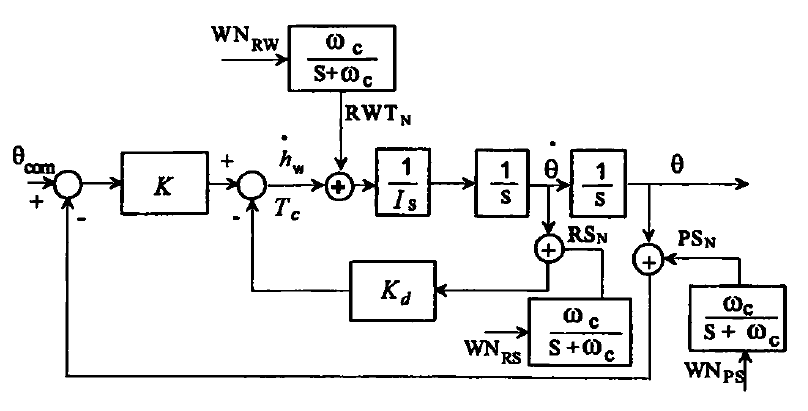
\includegraphics[width=8cm]{Figuras/ModeloControlAltitudSidi.png}
\caption{Esquema de control de altitud con ruido en los sensores y perturbaciones en la rueda de torque.}
\label{fig:ModeloControlAltitudSidi}
\end{figure}
\begin{figure}[h!]
\centering
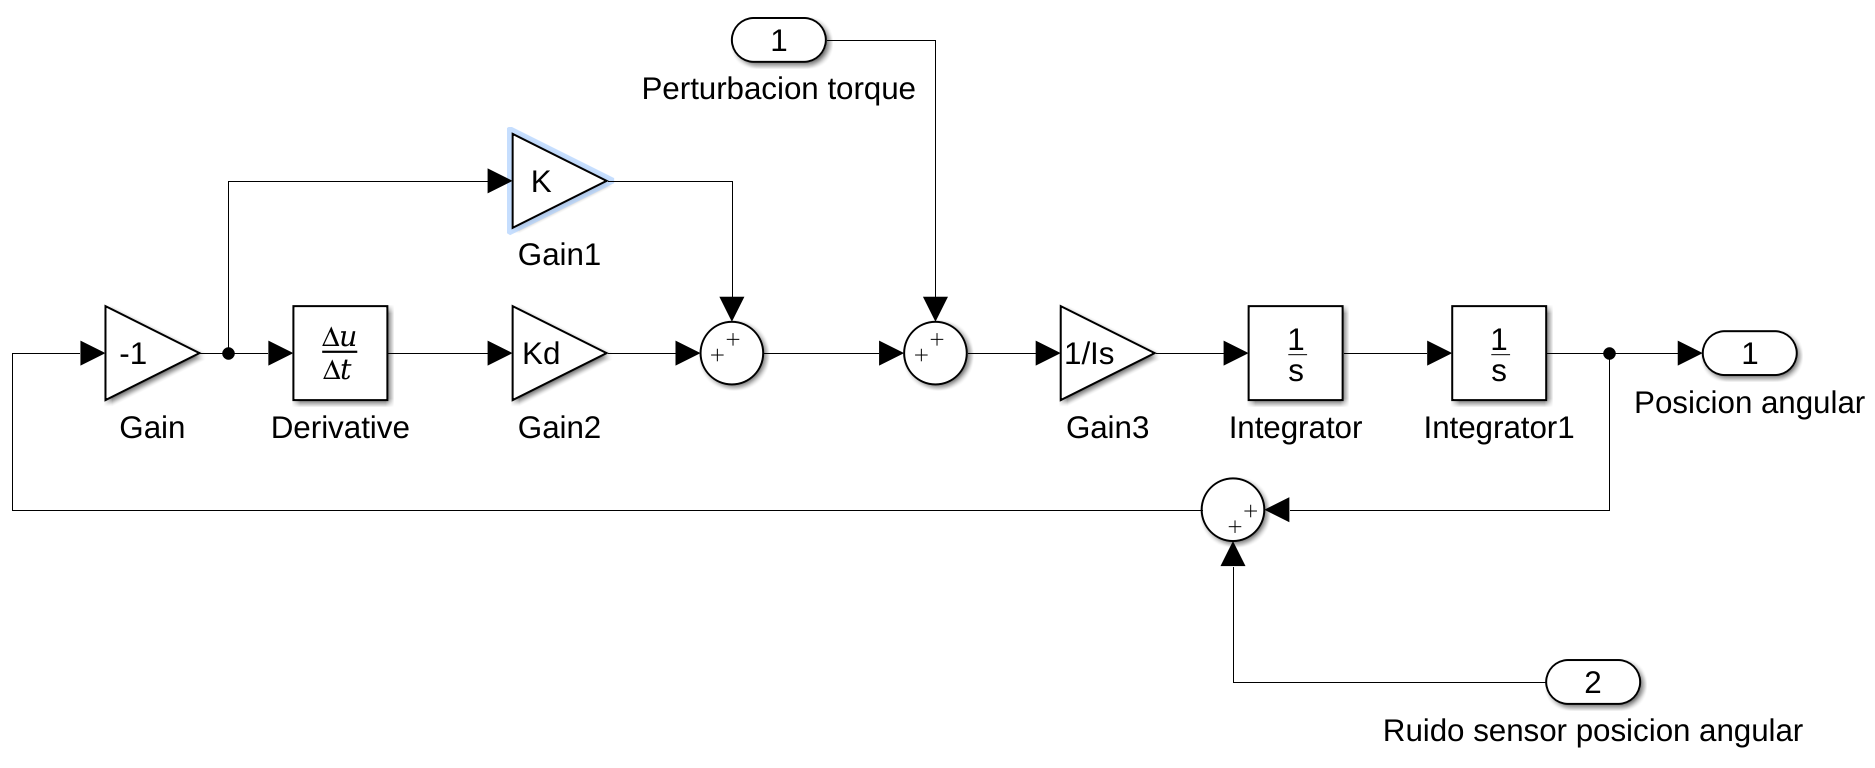
\includegraphics[width=8cm]{Figuras/SimulinkSistSinMedicionVelocidadAng.png}
\caption{Mismo sistema pero sin medición de la velocidad angular}
\label{fig:SimulinkSistSinMedicionVelocidadAng}
\end{figure}
\newpage
\section{MEMORIA TÉCNICA}
En referencia a la figura Nº\ref{fig:ModeloControlAltitudSidi} se tiene:
\begin{itemize}
\item $WN_{RS}$: ruido del sensor de velocidad angular. 
\item $WN_{PS}$: ruido del sensor de posición angular. 
\item $WN_{RW}$: ruido de torque inherente a la rueda de reacción.
\end{itemize}
De acuerdo a \cite{Sidi}, cada uno de estos tres ruidos es idealmente blanco, y por lo tanto tienen una densidad espectral de potencia (PSD) plana. Desafortunadamente, en la realidad el ruido blanco no existe. 
\\En cambio, se puede asumir que el ruido es coloreado; es decir, que su PSD varía en función de la frecuencia. Para ejemplificar esto en la Fig. Nº\ref{fig:ModeloControlAltitudSidi} se tienen los bloques de un filtro de primer orden con frecuencia de corte $\omega_c$, lo que no implica que los tres filtros posean el mismo valor de $\omega_c$.
\subsection{Funciones transferencia}
A partir de la Fig. Nº\ref{fig:ModeloControlAltitudSidi} considerando como entrada cada una de las entradas aleatorias y como salida la velocidad y la posición angular, se tienen las funciones trasferencia de las ecuaciones Ec.(\ref{ec:FTVelWNRS}), Ec.(\ref{ec:FTPosWNRS}), Ec.(\ref{ec:FTVelWNPS}), Ec.(\ref{ec:FTPosWNPS}), Ec.(\ref{ec:FTVelWNRW}) y Ec.(\ref{ec:FTPosWNRW}) para el sistema I:
\begin{equation}
\frac{\dot{\Theta}(s)}{WN_{RS}(s)}=-\frac{\omega_c}{s+\omega_c}\frac{2\xi\omega_ns}{s^2+2\xi\omega_ns+\omega_n^2}
\label{ec:FTVelWNRS}
\end{equation}
\begin{equation}
\frac{\Theta (s)}{WN_{RS}(s)}=-\frac{\omega_c}{s+\omega_c}\frac{2\xi\omega_n}{s^2+2\xi\omega_ns+\omega_n^2}
\label{ec:FTPosWNRS}
\end{equation}
\begin{equation}
\frac{\dot{\Theta}(s)}{WN_{PS} (s)}=-\frac{\omega_c}{s+\omega_c}\frac{\omega_n^2s}{s^2+2\xi\omega_ns+\omega_n^2}
\label{ec:FTVelWNPS}
\end{equation}
\begin{equation}
\frac{\Theta (s)}{WN_{PS} (s)}=-\frac{\omega_c}{s+\omega_c}\frac{\omega_n^2}{s^2+2\xi\omega_ns+\omega_n^2}
\label{ec:FTPosWNPS}
\end{equation}
\begin{equation}
\frac{\dot{\Theta}(s)}{WN_{RW} (s)}=\frac{\omega_c}{s+\omega_c}\frac{\frac{s}{I_s}}{s^2+2\xi\omega_ns+\omega_n^2}
\label{ec:FTVelWNRW}
\end{equation}
\begin{equation}
\frac{\Theta (s)}{WN_{RW} (s)}=\frac{\omega_c}{s+\omega_c}\frac{\frac{1}{I_s}}{s^2+2\xi\omega_ns+\omega_n^2}
\label{ec:FTPosWNRW}
\end{equation}
Donde:
\begin{equation}
\begin{cases}
I_s\, es\, dato \\
\xi = \frac{K_d}{2\sqrt{I_sK}} \\
w_n^2=\frac{K}{I_s}
\end{cases}
\end{equation}
Para el sistema II:
\begin{equation}
\frac{\Theta (s)}{WN_{PS} (s)}=\frac{\omega_c}{s+\omega_c}\frac{2\xi\omega_n+s+w_n^2}{s^2+2\xi\omega_ns+\omega_n^2}
\label{ec:FTPosWNPSII}
\end{equation}
\begin{equation}
\frac{\Theta (s)}{WN_{RW} (s)}=\frac{\omega_c}{s+\omega_c}\frac{\frac{1}{I_s}}{s^2+2\xi\omega_ns+\omega_n^2}
\label{ec:FTPosWNRWII}
\end{equation}
\subsection{Cálculo analítico del valor cuadrado medio}
\label{seccion:calculosValorCuadradoMedio}
Si se tiene un sistema LTI cuya función transferencia es $G(s)$ y se le aplica como entrada una señal ruidosa cuya función PSD es $S_i(s)$, la función PSD $S_o(s)$ de la salida de acuerdo a \cite{Grover} es:
\begin{equation}
S_o(s)=G(s)G(-s)S_i(s)
\end{equation}
Escribiendo a $S_o(s)$ como un cociente de polinomios:
\begin{equation}
S_o(s)=\frac{c(s)}{d(s)}\frac{c(-s)}{d(-s)}
\label{ec}
\end{equation}
Y bajo las hipótesis de que los ceros y polos de $c(s)/d(s)$ se hayan en el semiplano izquierdo y también que $d(s)$ no tiene raíces sobre el eje $j\omega$, se puede calcular el valor cuadrado medio como:
\begin{equation}
E\left(salida^2\right)=RMS^2=\frac{1}{2\pi j}\int_{-j\infty}^{j\infty}S_o(s)ds=\frac{1}{2\pi j}\int_{-j\infty}^{j\infty}\frac{c(s)}{d(s)}\frac{c(-s)}{d(-s)}ds
\label{ec:calculoMS}
\end{equation}
La potencia del resultado de la Ec.(\ref{ec:calculoMS}) se haya en la disponibilidad de tablas de integrales para la resolución de la integral. Estas se hayan en \cite{Grover}.
\\Aplicando este resultado a las funciones transferencia recién descriptas, se obtienen los valores cuadrados medios de la velocidad y de la posición para cada entrada.
\subsubsection{Entrada $WN_{RS}$}
Para el sistema I, utilizando la Ec.(\ref{ec:FTVelWNRS}) en la Ec.(\ref{ec:calculoMS}), se obtiene el valor cuadrado medio de la velocidad angular:
\begin{equation}
E\left( \dot{\Theta}^2\right)=\frac{\left(\xi\omega_n\omega_c \right)^2}{\xi\omega_n^3+2\xi^2\omega_n^2\omega_c+\xi\omega_c^2\omega_n}WN_{RS}
\end{equation}
Si se toma $$\lim_{\omega_c\to\infty}E\left( \dot{\Theta}^2\right)$$ se obtiene el valor de $E\left( \dot{\Theta}^2\right)$ para el caso ideal de ruido blanco. Se obtiene entonces:
\begin{equation}
\lim_{\omega_c\to\infty}E\left( \dot{\Theta}^2\right)=\xi\omega_nWN_{RS}
\label{ec:limiteVelWNRSI}
\end{equation}
Procediendo de manera análoga para la posición angular:
\begin{equation}
\begin{cases}
E\left( \Theta^2\right)=\frac{2\xi^3\omega_n\omega_c+\xi^2\omega_c^2}{\xi\omega_n^3+2\xi^2\omega_n^2\omega_c+\xi\omega_c^2\omega_n}WN_{RS}
\\
\\
\lim_{\omega_c\to\infty}E\left( \Theta^2\right)=\frac{\xi}{\omega_n}WN_{RS}
\end{cases}
\label{ec:limitePosWNRSI}
\end{equation}
\subsubsection{Entrada $WN_{PS}$}
Para el sistema I:
\begin{equation}
\begin{cases}
E\left( \dot{\Theta}^2\right)=\frac{\omega_n^4\omega_c^2}{4\left( \xi\omega_n^3+2\xi^2\omega_n^2\omega_c+\xi\omega_n\omega_c^2 \right)}WN_{PS}
\\
\\
\lim_{\omega_c\to\infty}E\left( \dot{\Theta}^2\right)=\frac{\omega_n^3}{4\xi}WN_{PS}
\end{cases}
\label{ec:limiteVelWNPSI}
\end{equation}
\begin{equation}
\begin{cases}
E\left( \Theta^2\right)=\frac{2\xi\omega_n^3\omega_c+\omega_n^2\omega_c^2}{4\left( \xi\omega_n^3+2\xi^2\omega_n^2\omega_c+\xi\omega_n\omega_c^2 \right)}WN_{PS}
\\
\\
\lim_{\omega_c\to\infty}E\left( \Theta^2\right)=\frac{\omega_n}{4\xi}WN_{PS}
\end{cases}
\label{ec:limitePosWNPSI}
\end{equation}
Para el sistema II:
\begin{equation}
E\left( \Theta^2\right)=\frac{c_1^2d_0+c_0^2d_2}{2d_0\left( d_1d_2-d_0d_3\right)} WN_{RW}
\end{equation}
Donde:
\begin{equation}
\begin{cases}
c_0=\omega_n^2\omega_c \\
c_1=2\xi\omega_n\omega_c \\
d_0=\omega_c\omega_n^2 \\
d_1=\omega_n^2+2\xi\omega_c\omega_n \\
d_2=2\xi\omega_n+\omega_c \\
d_3=1
\end{cases}
\end{equation}
\subsubsection{Entrada $WN_{RW}$}
Para el sistema I:
\begin{equation}
\begin{cases}
E\left( \dot{\Theta}^2\right)=\frac{\omega_c^2}{4I_s^2\left( \xi\omega_n^3+2\xi^2\omega_n^2\omega_c+\xi\omega_n\omega_c^2 \right)}WN_{RW}
\\
\\
\lim_{\omega_c\to\infty}E\left( \dot{\Theta}^2\right)=\frac{1}{4\xi I_s^2 \omega_n}WN_{RW}
\end{cases}
\label{ec:limiteVelWNRWI}
\end{equation}
\begin{equation}
\begin{cases}
E\left( \Theta^2\right)=\frac{2\xi\omega_n\omega_c+\omega_c^2}{4I_s^2\omega_n^2\left( \xi\omega_n^3+2\xi^2\omega_n^2\omega_c+\xi\omega_n\omega_c^2 \right)}WN_{RW}
\\
\\
\lim_{\omega_c\to\infty}E\left( \Theta^2\right)=\frac{1}{4\omega_n^3 I_s^2\xi}WN_{RW}
\end{cases}
\label{ec:limitePosWNRWI}
\end{equation}
Para el sistema II:
\begin{equation}
E\left( \Theta^2\right)=\frac{c_0^2d_2}{2d_0\left( d_1d_2-d_0d_3\right)} WN_{RW}
\end{equation}
Donde:
\begin{equation}
\begin{cases}
c_0=\frac{\omega_c}{I_s} \\
d_0=\omega_c\omega_n^2 \\
d_1=\omega_n^2+2\xi\omega_c\omega_n \\
d_2=2\xi\omega_n+\omega_c \\
d_3=1
\end{cases}
\end{equation}
\subsection{Simulaciones}
Para poder realizar simulaciones en \textit{Simulink} es necesario primero comprender como utilizar el bloque \textit{Band Limited White Noise} (BLWN), que como su nombre lo indica, genera ruido blanco con un ancho de banda limitado. Haciendo uso de este, se simulan las señales aleatorias.
Los parámetros que requiere son:
\begin{itemize}
\item Noise power.
\item Sample time.
\item Seed: una semilla para generar números aleatorios.
\end{itemize}
Los primeros dos parámetros definen el valor RMS del ruido:
\begin{equation}
RMS=\sqrt{\frac{Noise\,power}{Sample\,time}}
\end{equation}
Por otra parte, si se tiene ruido blanco cuya densidad espectral de potencia tiene ancho de banda limitado como el de la Fig. Nº\ref{fig:PSDBLWNTeorico}, se sabe que su valor RMS es:
\begin{equation}
RMS=\sqrt{2fA}
\label{ec:RMSTeorico}
\end{equation}
\begin{figure}[h!]
\centering
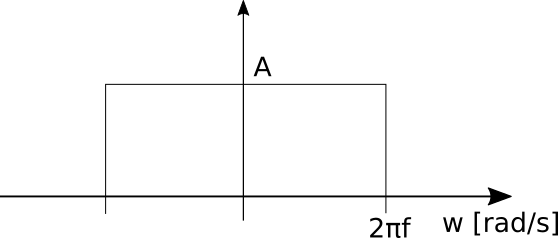
\includegraphics[width=8cm]{Figuras/PSDBLWNTeorico.png}
\caption{Densidad espectral de potencia de ruido blanco con ancho de banda limitado}
\label{fig:PSDBLWNTeorico}
\end{figure}
Desafortunadamente, si uno pretende definir un ruido de acuerdo a la Fig. Nº\ref{fig:PSDBLWNTeorico}, no es directo asociarlo al bloque BLWN como $Noise\,power=A$ y $Sample\,time=1/f$. Entonces, teniendo presente que uno desea construir un ruido con una PSD como la de la Fig. Nº\ref{fig:PSDBLWNTeorico}, ¿cómo se definen los parámetros del bloque BLWN?. 
\\Llamando $A$ y $T_S$ los parámetros \textit{Noise power} y \textit{Sample time} del bloque BLWN, resulta $RMS=\sqrt{\frac{A}{T_S}}$. A su vez, las Figs. Nº\ref{fig:PSDBLWNTeoricoOpcion1} y Nº\ref{fig:PSDBLWNTeoricoOpcion2} muestran dos opciones que de acuerdo a la Ec.(\ref{ec:RMSTeorico}) también tienen $RMS=\sqrt{\frac{A}{T_S}}$. De acuerdo a la práctica adquirida y a que los valores de las ecuaciones del valor cuadrado medio (sección \ref{seccion:calculosValorCuadradoMedio}) depende del valor de $A$, se debe utilizar la PSD de la Fig. Nº\ref{fig:PSDBLWNTeoricoOpcion1}.
\begin{figure*}[t!]
    \centering
    \begin{subfigure}[t]{0.5\textwidth}
        \centering
        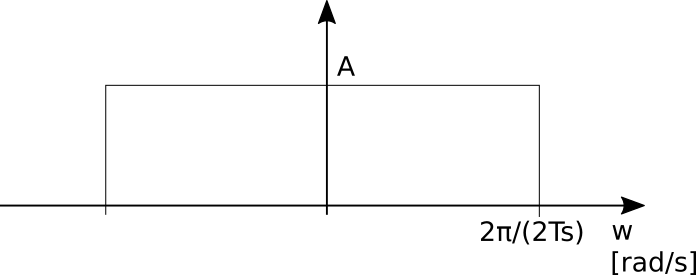
\includegraphics[width=8cm]{Figuras/PSDBLWNTeoricoOpcion1.png}
        \caption{}
        \label{fig:PSDBLWNTeoricoOpcion1}
    \end{subfigure}%
    \begin{subfigure}[t]{0.5\textwidth}
        \centering
        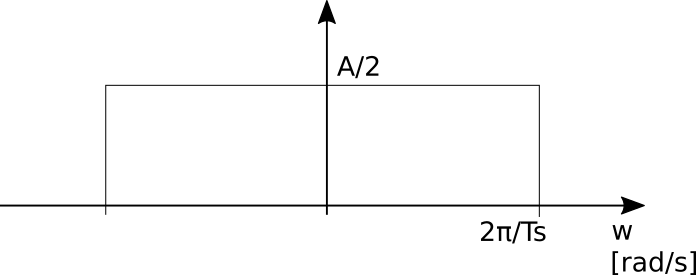
\includegraphics[width=8cm]{Figuras/PSDBLWNTeoricoOpcion2.png}
        \caption{}
        \label{fig:PSDBLWNTeoricoOpcion2}
    \end{subfigure}%
    ~ 
    \caption{Dos opciones para relacionar los parámetros del bloque BLWN con la PSD de la Fig. Nº\ref{fig:PSDBLWNTeorico}.}
    \label{}
\end{figure*}
\par En la tabla Nº\ref{tabla:parametros} se muestran los valores adoptados de $I_s$, $\xi$ y $\omega_n$ y los valores calculados de $K$ y $K_d$. A su vez, se toma $\omega_c=100\omega_n=1\,rad/s=0.16\,Hz$ y se pretende que la PSD del ruido generado por el bloque BLWN tenga un ancho de banda de banda de 100 veces $\omega_c\,[Hz]$. De esta manera, $Sample\,time=\frac{1}{2*100*\omega_c\,[Hz]}=0.0314\,s$.
\begin{table}[h!]
\centering
\caption{Valores adoptados de $I_s$, $\xi$ y $\omega_n$ y valores calculados de $K$ y $K_d$.}
\label{tabla:parametros}
\begin{tabular}{|c|c|}
\hline
Parámetro & Valor \\ \hline
$I_s$ & $1000\,kg\,m^2$  \\ \hline
$\xi$ & $0.7$  \\ \hline
$\omega_n$ & $0.01\,rad/s$ \\ \hline
$K$ & $0.1$ \\ \hline
$K_d$ & $14$ \\ \hline
\end{tabular}
\end{table}
\par Los valores adoptados del desvío o valor RMS de las distintas señales aleatorias se muestran en la tabla Nº\ref{tabla:RMSruidos}.
\begin{table}[h!]
\centering
\caption{Valores adoptados para el desvío de las distintas señales aleatorias}
\label{tabla:RMSruidos}
\begin{tabular}{|c|c|}
\hline
Señal aleatoria & Desvío \\ \hline
Posición angular&$0.1\,rad$ \\ \hline
Velocidad angular&$0.1\,rad/s$ \\ \hline
Torque&$1\,Nm$ \\ \hline
\end{tabular}
\end{table}
\subsection{Resultados}
En la tablas Nº\ref{tabla:ResultadosSistI} y Nº\ref{tabla:ErroresSistI} se muestran los resultados y errores para las simulaciones del sistema I, y en la tabla Nº\ref{tabla:ResultadosSistII} los resultados y errores del sistema II. Los errores se calculan respecto del resultado de la simulación. 
\\El tiempo de simulación se ajusto en cada una para permitir que el sistema evolucione y así lo haga también el valor esperado de la salida considerada. De lo contrario, se tienen errores mayores. A su vez, se requieren \textit{grandes} tiempos de simulación debido a la respuesta \textit{lenta} del sistema ($\omega_n=0.01\,rad/s$); y cuánto mayor el tiempo de simulación, mayor el tiempo que requiere la ejecución de la misma. 
\begin{table}[h!]
\centering
\caption{Resultados del sistema I}
\label{tabla:ResultadosSistI}
\begin{tabular}{|c|c|c|c|c|c|c|}
\hline
Entrada  & $WN_{RS}$ & $WN_{RS}$& $WN_{PS}$& $WN_{PS}$& $WN_{RW}$&$WN_{RW}$\\ \hline
T. de sim.&$10000\,s$&$10000\,s$&$100000\,s$&$100000\,s$&$100000\,s$&$100000\,s$ \\ \hline
Parámetro & $E\left( \dot{\Theta}^2 \right)$ & $E\left( \Theta^2\right)$& $E\left( \dot{\Theta}^2 \right)$ & $E\left( \Theta^2\right)$& $E\left( \dot{\Theta}^2 \right)$ & $E\left( \Theta^2\right)$  \\ \hline
Cálculo explícito&$2.17\,10^{-6}$&$0.022$&$1.11\,10^{-}$&$1.12\,10^{-6}$&$1.11\,10^{-6}$&$0.012$\\ \hline
$\lim_{\omega_c\to\infty}$&$2.2\,10^{-6}$&$0.022$&$1.12\,10^{-10}$&$1.22\,10^{--6}$&$1.12\,10^{-6}$&$0.0112$ \\ \hline
Simulación&$2.05\,10^{-6}$&$0.0228$&$1.16\,10^{-10}$&$1.24\,10^{-6}$&$1.16\,10^{-6}$&$0.012$ \\ \hline
%&&&&&& \\ \hline
\end{tabular}
\end{table}
\begin{table}[h!]
\centering
\caption{Errores del sistema I}
\label{tabla:ErroresSistI}
\begin{tabular}{|c|c|c|c|c|c|c|}
\hline
Entrada  & $WN_{RS}$ & $WN_{RS}$& $WN_{PS}$& $WN_{PS}$& $WN_{RW}$&$WN_{RW}$\\ \hline
Parámetro & $E\left( \dot{\Theta}^2 \right)$ & $E\left( \Theta^2\right)$& $E\left( \dot{\Theta}^2 \right)$ & $E\left( \Theta^2\right)$& $E\left( \dot{\Theta}^2 \right)$ & $E\left( \Theta^2\right)$  \\ \hline
Cálculo explícito&$5.98\%$&$3.46\%$&$4.33\%$&$9.53\%$&$3.49\%$&$0.19\%$ \\ \hline
$\lim_{\omega_c\to\infty}$&$7.47\%$&$3.45\%$&$2.98\%$&$9.52\%$&$2.23\%$&$0.2\%$\\ \hline
%&&&&&& \\ \hline
\end{tabular}
\end{table}
\begin{table}[h!]
\centering
\caption{Resultados y erroresdel sistema II}
\label{tabla:ResultadosSistII}
\begin{tabular}{|c|c|c|}
\hline
Entrada  &  $WN_{PS}$& $WN_{RW}$\\ \hline
T. de sim.&$10000\,s$&$100000\,s$ \\ \hline
Parámetro & $E\left( \Theta^2 \right)$ & $E\left( \Theta^2\right)$\\ \hline
Cálculo explícito&$3.29\,10^{-4}$&$0.0112$\\ \hline
Simulación&$3.51\,10^{-4}$&$0.0112$\\ \hline
Error &$6.55\%$&$0.19\%$ \\ \hline
%&&&&&& \\ \hline
\end{tabular}
\end{table}

\newpage
\section{CONCLUSIONES}
El presente trabajo permitió comprender como calcular la respuesta de un sistema LTI frente a entradas estocásticas. Para poder llevar a cabo las simulaciones primero fue necesario entender el funcionamiento del bloque BLWN de Simulink y cómo asociarlo a la densidad espectral de potencia del ruido que se pretende simular. De hecho, en primera instancia había mal interpretado el funcionamiento del bloque, lo que significó varios resultados erróneos y un gran malgasto del tiempo invertido.  
\par Los resultados de las simulaciones ratifican los resultados de los valores esperados calculados mediante las ecuaciones de la sección \ref{seccion:calculosValorCuadradoMedio} dentro de un margen de error. En primera instancia es esperable, puesto que estas ecuaciones tienen como hipótesis que el ruido en la entrada del sistema es blanco. Como se mencionó anteriormente, este en realidad no existe y tampoco se puede simular. De todas maneras, al utilizar un ancho de banda para el ruido lo suficientemente mayor al ancho de banda del sistema, es una hipótesis adecuada.
\\ También, otro factor de importancia en el error es el tiempo de simulación. Cuánto mayor sea este, menor será el error. De todas maneras, el valor esperado del valor cuadrado medio de la salida de interés alcanza un valor estacionario, por lo que el error nunca convergirá a cero. 
\\Otra consideración respecto al tiempo de simulación, es la relación de este con el tiempo real que le toma a la computadora llevarla a cabo. En el ejemplo que se trató, esto es un tanto desfavorable por el bajo ancho de banda del sistema (proporcional a $\omega_n$). De esta manera, cada vez que se requería un tiempo de simulación mayor, se debía esperar varios minutos a que la computadora resuelva. 
\par Finalmente, una aplicación provechosa de lo aquí aprendido es en el diseño del sistema. Si se observan las ecuaciones Ec.(\ref{ec:limiteVelWNRSI}), Ec.(\ref{ec:limitePosWNRSI}), Ec.(\ref{ec:limiteVelWNPSI}), Ec.(\ref{ec:limitePosWNPSI}), Ec.(\ref{ec:limiteVelWNRWI}) y Ec.(\ref{ec:limitePosWNRWI}) en los casos que $\omega_c$ tiende a infinito, el valor esperado de cada salida de interés depende de $\omega_n$. Dado  que $\omega_n$ da idea del ancho de banda del sistema, se puede hallar encontrar un valor para este que minimice la respuesta del ruido. Esta solución será de compromiso puesto que la dependencia de las ecuaciones citadas respecto de $\omega_n$ en algunos casos es proporcional y en otros inversamente proporcional. 
\newpage
\bibliographystyle{asmems4}
\bibliography{biblio}
\end{document}
%que